\documentclass[font=10pt]{article}
\usepackage[left=3cm,right=3cm,top=3cm,bottom=3cm]{geometry}
\usepackage{graphicx}
\usepackage{float}
%\setcounter{tocdepth}{4}
\graphicspath{ {./images/} }
\begin{document}

  \begin{titlepage}
    \centering
    \title{\textbf{INFO3406 Assignment Stage 2}}
    \author{
      Nick Zhou 460363707\\
      Linzi Zhu 46xxxxxxx
    }
    \date{October 2018}
    \maketitle
    
\includegraphics[width=5cm]{usyd}
  \end{titlepage}

  \begin{tableofcontents}
    \tableofcontents
  \end{tableofcontents}

  \section{Section 1: Setup}
    \subsection{Research Questions and Hypothesis}
    % State your research question(s). State null and alternative hypotheses
      \subsubsection{Research Questions}

      The research questions which we will attempt to answer is:
      \begin{enumerate}
        \item Is there a link between the emotional response a movie’s title evokes (sight unseen) and the movies eventual gross revenue?
        \item Using these models, can we train a predictor to assess the value of a title for any given movie?
      \end{enumerate}

      \subsubsection{Hypotheses}

      \underline{Hypotheses}
      \begin{itemize}
        \item H0 (the null Hypothesis): Lexicon usage in movie titles \textit{does not have a statistically significant effect} on the performance of a movie.
        \item H1 (the alternative Hypothesis): Lexicon usage in movie does \textit{has a statistically significant effect} on the performance of a movie.
      \end{itemize}

    \subsection{Reliability}
    % Describe how you will quantify reliability e.g. significance testing, confidence intervals. If appropriate, describe how you will measure effectiveness e.g. regression r-square, clustering V-measure, classification f1-score.

    \subsection{Dataset}
    % Identify datasets and the data you derived from them
    The dataset was derived from the previous stage.

  \section{Section 2: Approach}
  Approach...
  \section{Section 3: Results}
  The results to appear to indicate that...
  \section{Conclusion}
  There was no evidence to support the alternative hypothesis and as a result we retain the null hypothesis\
  which is that there is effect on movie performance based on their lexicon usage in titles.

  \appendix
  \section{Graphs}
  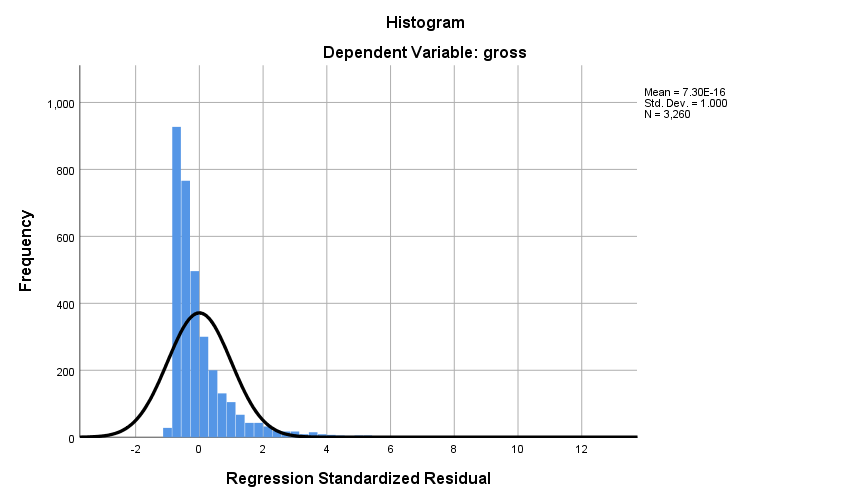
\includegraphics[width=10cm]{graph1}
  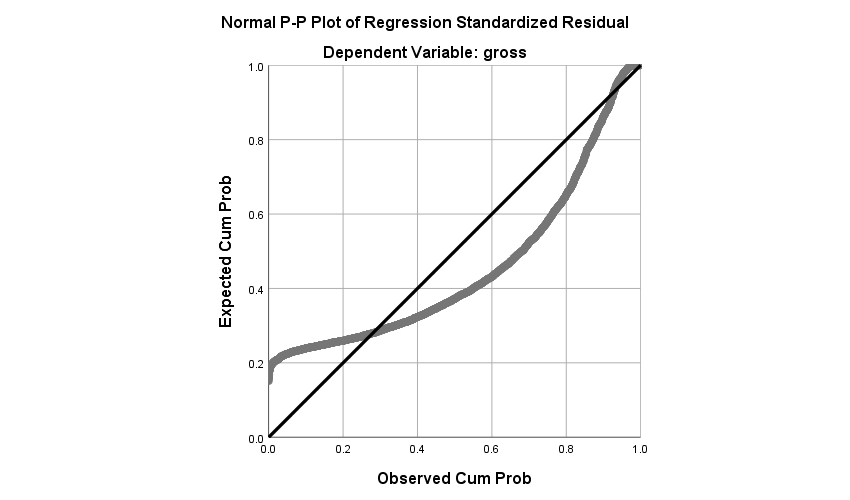
\includegraphics[width=10cm]{graph2}
  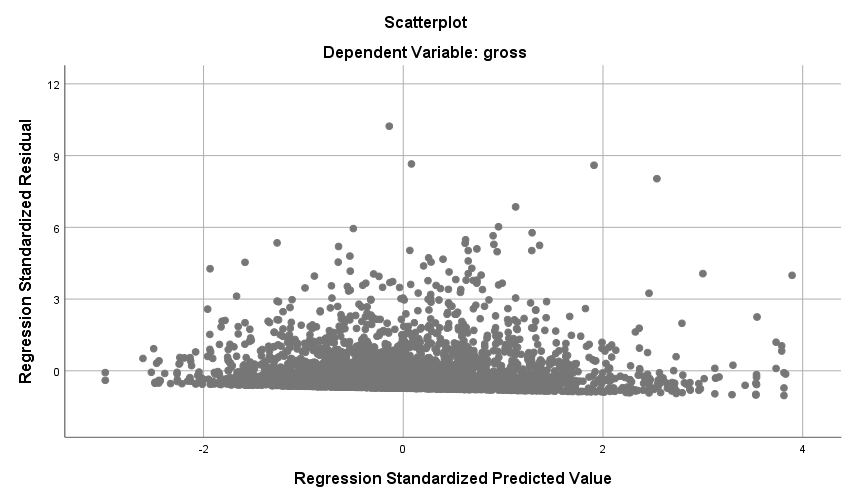
\includegraphics[width=10cm]{graph3}

\end{document}
